\documentclass[10pt,twocolumn]{IEEEtran}

\usepackage[linesnumbered,lined,boxed,commentsnumbered, noend, noline]{algorithm2e}
\usepackage{graphicx}
\usepackage{xcolor}
\usepackage{soul}

\newcommand{\hlc}[2][yellow]{{%
    \colorlet{foo}{#1}%
    \sethlcolor{foo}\hl{#2}}%
}

\title{Analyzing Algorithmic Patterns Based on Real Coding Interview Questions}
\author{Ian Dempsey}
%\hlc[cyan!50]{_____} -> put in the stuff to be highlighted inside the {}

\begin{document}

\maketitle
\pagenumbering{gobble}
\newpage
\pagenumbering{arabic}

\section{General Patterns for Analysis}
\subsection{Palindrome}
Palindromes are extremely useful for searching algorithms, as Palindromes are meant to be the same in both directions, one can easily discover if the input is an actual palindrome. This is helpful for searching because one can search and find the odd character out, or the unique piece of data in some text. This style of algorithm is also space efficient, they normally have a space analysis of O(n/2) as the algorithm works over two elements of the input at a time. The basic approach of a Palindrome algorithm is to work inwards with both pointers starting at either end of the input and constantly moving towards one another and comparing if the elements are the same.\\  
The following description is a general algorithm for solving the palindrome problem which is a common problem in Java and other languages. This approach can be used to solve numerous other problems by altering the inside of the loop.
Pseudocode:
\IncMargin{1em}
\begin{algorithm}
	\SetAlgoLined
	\KwData{Given input of characters, S}
	\KwResult{Boolean}
	initialization\;
	$leftIndex  \longleftarrow $S[0]\;
	$rightIndex \longleftarrow $S.length-1\;
	\While{leftIndex $<$ rightIndex}{
	
	compare leftIndex with rightIndex\;
	\If{leftIndex !=rightIndex}{
		return false\;
	}
	 leftIndex++\;
	rightIndex++\;
}
return true\;
\caption{The Palindrome Algorithm}
\end{algorithm}\DecMargin{1em}

Whilst studying and working on this project I have answered a number of questions from Leetcode.com which I was able to solve using an altered version of the above Palindrome pattern. Leetcode question 1 TwoSum is one example of these questions. This question is described as: \textit{Given an array of integers, return indices of the two numbers such that they add up to a specific target. You may assume that each input would have exactly one solution, and you may not use the same element twice.} The following pseudocode is my answer to this question. In it I have taken the basic idea of the Palindrome algorithm of having two pointers used for looking through the input data, but I have altered the way these two pointers behave.In this pseudocode I have highlighted any differences in blue.
\IncMargin{1em}
\begin{algorithm}
	\SetAlgoLined
	\KwData{Array of integers nums, target S}
	\KwResult{Indices i,j}
	$leftIndex  \longleftarrow $S[0]\;
	$rightIndex \longleftarrow $S.length-1\;
	\While{leftIndex $<$ rightIndex}{
	\hlc[cyan!50]{Sort the input array nums\;}\\
	\uIf{\hlc[cyan!50]{nums[leftIndex]+nums[rightIndex] $>$ S}}{
		\hlc[cyan!50]{rightIndex$--$\;}
	}\uElseIf{\hlc[cyan!50]{nums[leftIndex]+nums[rightIndex]$<$S}}{
		\hlc[cyan!50]{leftIndex++\;}
	}\Else{
		\hlc[cyan!50]{return leftIndex, rightIndex\;}
	}
     }return 0\;
\caption{LeetCode Q1 TwoSum}
\end{algorithm}\DecMargin{1em}\\
As can be seen from the above answer, the main differences are the conditionals inside the while loop. Instead of the normal approach of a Palindrome where one checks if the two elemts are equal, and if so moves the two pointers are moved at the same time towards eachother, I have changed the condisitionals such that instead of moving both of these pointers together at the same time, I only ever move one pointer at a time. Depending on the result of adding the two current elements at each pointer together. If the total from adding the two integers together was greater than the target sum, then I knew that I had to move the right-pointer left once, as this would allow me to have a smaller sum and potentially the correct sum. If on the other hand the sum was smaller than the total, I would only move the left-pointer right once and add the two elements and get a new result. This process was repeated until the target sum was found, or until the two pointers crossed which meant the target was not found.
\subsection{Merge Sort}
Merge Sort is a very powerful algorithm. It is more efficient than most styles of insertion, with a time analysis of $O(n * log_{n})$, whereas insertion is $O(n^2)$. The idea of merge sort is to divide an array or some input in half and then sort each half before joining it back together. They do not have to be the same size which is useful.  \\
Merge Sort uses the idea of divide and conquer, this means the list to be sorted should be divided up into equal parts first, then these new smaller parts should be sorted individually first before recreating the full list.
Pseudocode:
\IncMargin{1em}
\begin{algorithm}
	\SetAlgoLined
	\KwData{List of unsorted data}
	\KwResult{Sorted List}
 	\eIf{ length of A is 1}{ return 1}
  	{Split A into two halves , L and R. Repeat until size of part =1\\
  	Sort each part individually \\
  	Merge with another subdivided section into B, the sorted list\\ 
  	Return B, the sorted structure}
\caption{The Merge Sort Algorithm through Recursion}
\end{algorithm}\DecMargin{1em}

\subsection{Graphs}
Graphs are common in our lives. News media use them to help us visualize certain statistics. Though these are not the graphs that are studied by Computer Scientists. Graphs studied by Computer Scientists and Mathematicians are usally based on the tree structure, and the relationships among data elements. A tree is just one of the special types of graphs that can be studied, where the parent-child relationship is used to organise data. In this section I have focused on the Tree Abstract Data Type, Breadth-First Traversal, Depth-First Traversal and Graphs in general. \\
\subsubsection{Trees}
Trees are one of the most powerful styles of data structures for processing data, this is because they allow rapid searching and fast insetion/deletion of a node. Trees are made up of Nodes, these are just basic Objects which hold some data and have a key. This key allows one to determine where this Node should be in the tree. The important distinction here with these Nodes in comparison to other Nodes used in various data structures, is that these Nodes contain references to children instead of just the next Link. Each Node has exactly one parent, but can many children. There is a special style of Trees known as a Binary Tree. This is a Tree which has between 0 and 2 children. The first Node in a tree is the Root, and it is possible to traverse to any Node in the Tree from this Root Node.
With Trees the main function one must take care of is how to traverse them. There are three basic styles of traversal: inorder, preorder and postorder. Inorder visits every Node in ascending order based on their key values. Preorder is where the root is visited first, followed by it's left subtree and then it's right subtree. Finally, postorder is where the left subtree is followed by the right subtree and then the root. \\
The following is an example of how one might search for a particular Node in a Tree.
Pseudocode:
\IncMargin{1em}
\begin{algorithm}
	\SetAlgoLined
	\KwData{Given a key to search for}
	\KwResult{The desired Node, or null}
	initialization\;
	$Node current \longleftarrow$root\;
	\While{current.data is not key}{
		\If{current is null}{return null\;}
		\eIf{current.data $>$ key}{
			move left on the tree\;
		}{
		move right on the tree\;
		}
	}
return current\;
\caption{Finding a specific Node in a tree based on the key}
\end{algorithm}\DecMargin{1em}
\\
\IncMargin{1em}
\begin{algorithm}
	\SetAlgoLined
	\SetKwFunction{postOrder}{postOrder}
	\Indm\postOrder{$Node localRoot$}
	%\KwData{Node localRoot}
	%\KwResult{Print out in PostOrder}
	\\
		\If{localRoot $!=$ null}{
		\postOrder(localRoot leftChild)\\
		\postOrder(localRoot rightChild)\\
		Print(localRoot data)\;}	
\caption{Basic Tree Traversal using PostOrder Traversal}
\end{algorithm}\DecMargin{1em}
\\
Leetcode question 104, \textit{Maximum Depth of Binary Tree}, is an example of a problem where I used the basic tree traversal styles to solve the question.The problem description is given as: \textit{Given a binary tree, find its maximum depth.The maximum depth is the number of nodes along the longest path from the root node down to the farthest leaf node.} In this algorithm I used postorder traversal. Pseudocode can be found in Algorithm 6 of this paper.\\
\IncMargin{1em}
\begin{algorithm}
	\SetKwFunction{maxDepth}{maxDepth}
	\Indm\maxDepth{$TreeNode  localRoot$}\\
	\SetAlgoLined
	%\KwData{Node localRoot}
	%\KwResult{Print out in PostOrder}
		\If{\hlc[cyan!50]{localRoot $==$ null}}{\hlc[cyan!50]{ return 0\;}}
		\hlc[cyan!50]{int ldepth $=$}\hlc[cyan!50]{\maxDepth}\hlc[cyan!50]{(localRoot leftChild)}\;
		\hlc[cyan!50]{int rdepth $=$}\hlc[cyan!50]{ \maxDepth}\hlc[cyan!50]{(localRoot rightChild)}\;
		\If{\hlc[cyan!50]{ldepth $>$ rdepth}}{
		\hlc[cyan!50]{return ldepth+1}
		}\Else{\hlc[cyan!50]{return rdepth+1}}
\caption{Leetcode Q104 Max. Depth of Binary Tree}
\end{algorithm}\DecMargin{1em}
\\
As highlighted above, the key diference is inside the if statement. I have changed the conditional itself as it is the base case to stop the recursive execution. I have created a variable \textit{ldepth} which is the total depth of the left subtree. This is a recursive call on the leftChild of the current node. Line 4 will execute until it can't go left anymore, if it reaches null it will try to go right once, and then return going left. This is repeted until both calls return null. It then will go back all the way up until we reach the first call to go left, and set this summation of steps to ldepth. It then performs this same process but on the right subtree of the current node(which is the original node given), and set it to the variable \textit{rdepth}. Finally there is a conditional checking if ldepth is greater than rdepth. If so it returns ldepth+1,or it returns rdepth+1. This+1 is required as I need to take into account the root node's level, if I didn't take this into account my answer would always be one less than the actual depth of the tree. The major similarities between the postorder algorithm and this solution is the way I went down the left subtree first, then the right subtree and finally to take into account the root I added one to the height. This particular way of traversing the tree, left-right-root, is exactly how postorder traversal is performed.
\\
\subsubsection{Breadth-First Traversal}
This is a special way to visit the nodes in a tree, the ordering in this traversal pattern is to visit the root node, then move onto the children of the root node, printing each child in turn. It then will repeat this for each child of these nodes.Figure 1 shows the nodes in numerical order of visitation when using Breadth-First Traversal. \\
\begin{figure}[h]
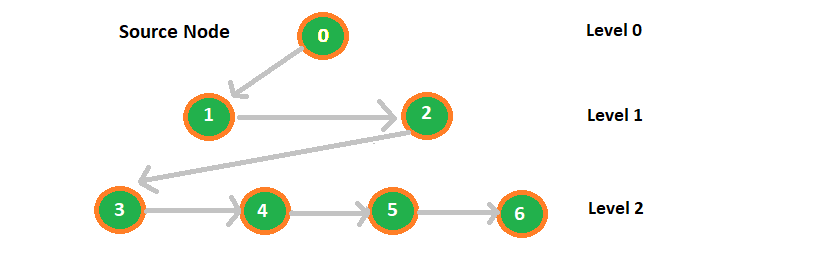
\includegraphics[width=0.6\textwidth]{bfs.png}
\caption{Breadth-First Traversal}
\end{figure}
 \\
\subsubsection{Depth-First Traversal}
This is a second way of visiting nodes in a tree. This pattern involves starting at the root node, then going to the left most child, then repeating this movement until the traversal reaches a leaf node (a node which has no children), then it will move back up one node and try to visit the next child node of this current node. It repeats this until the traversal finds no univisited node. Figure 2 shows the nodes in numerical order of visitation when using Depth-First Traversal. 
\begin{figure}[h]
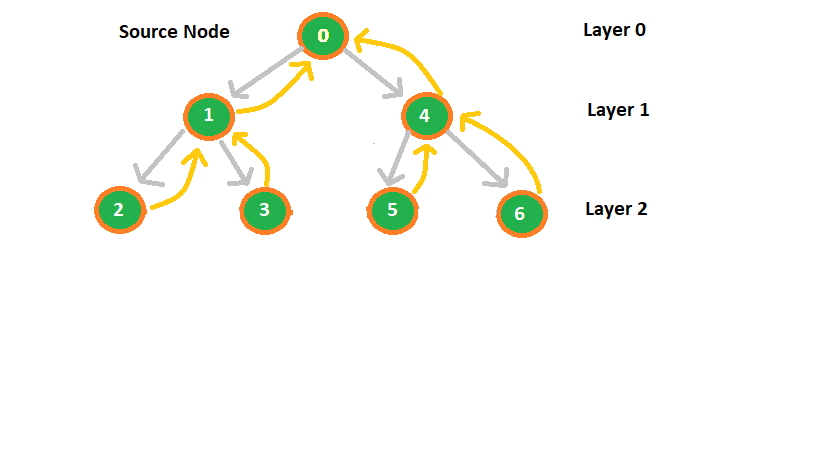
\includegraphics[width=0.6\textwidth]{dfs.png}
\caption{Depth-First Traversal}
\end{figure}
\end{document}